
\subsection{Allocator Versions}

To facilitate the support for multiple versions of the allocator with a configurable design, the primary TLSF implementation has been abstracted into a base class named \texttt{TLSFBase}. The base class implements all parts described in the TLSF design except for the \texttt{free()} method, which varies greatly between use-cases and should therefore be implemented optimally for every new configuration. For each configuration, the base class enables the user to specify the allocator's behavior through a set of configuration variables, which includes:

\begin{enumerate}
  \item Number of first- and second-level indexes.
  \item Whether to use second-level or not.
  \item Minimum block size.
  \item Whether to use deferred coalescing.
  \item Block header length.
\end{enumerate}

\subsection{New Bitmap Design}

Summarizing the insight from Section~\ref{sec:adaptations:reduced_allocation_range} regarding the number of required first- and second-levels, desire to use a single 64-bit bitmap and large-list, we can construct a new bitmap representation, as shown in Figure~\ref{fig:bitmap_flattening}. The new bitmap disregards the literal notion of ``Two Level'' from Two Level Segregated Fit and flattens the first- and second-level bitmaps to a single bitmap. The new bitmap is indexed using the formula: 
\[
    \text{bitmap\_index($f, s$)} = f \cdot 4 + s
\]
where $f$ and $s$ are the first- and second-level indexes respectively. Additionally, the lowest size classes have been placed at the least significant bits of the bitmap to make searching for the next non-empty free-list efficient using the find-first-set bit instruction.

\begin{figure}[H]
    \centering
    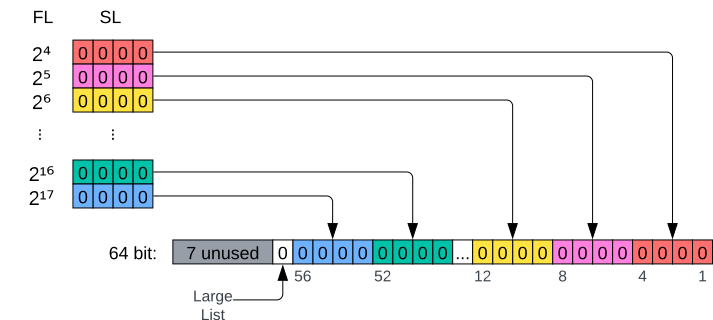
\includegraphics[width=1\textwidth]{figures/bitmap_flattening.png}
    \caption{Flattening of the 2D-matrix representation of TLSF bitmaps into a single 64-bit value. The first-level bitmap is disregarded in favor of indexing the new flattened bitmap using the first-level value instead. The number of first-levels are 14, indicated by bits of the same color belonging to the same first-level. The number of second-levels are 4, as indicated by the same number of colored bits.}
    \label{fig:bitmap_flattening}
\end{figure}

The correlation between the bitmap and the free-lists is depicted in Figure~\ref{fig:bitmap_relationship}, adhering closely to the original TLSF design. However, the adaptation now efficiently determines the relevant free-list by looking in the single bitmap, not two bitmaps as in the original design.

\begin{figure}[H]
    \centering
    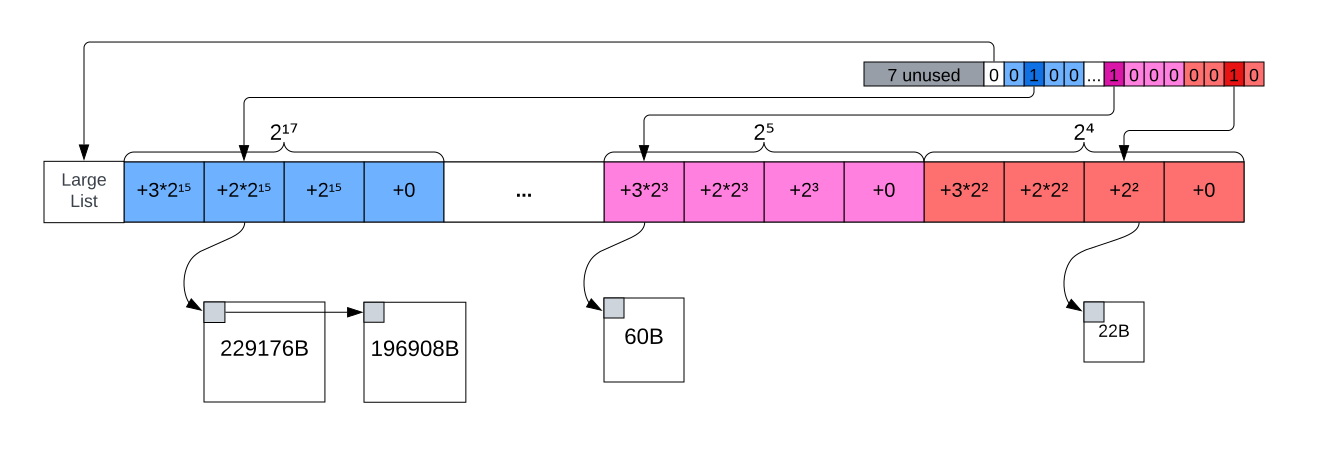
\includegraphics[width=1\textwidth]{figures/bitmap_relationship.png}
    \caption{Relationship between the new bitmap representation and accessing the corresponding free-lists.}
    \label{fig:bitmap_relationship}
\end{figure}

\subsection{Block Header Adjustments and 0-byte Header}

The block header, as used in the reference implementation, is shown in Figure~\ref{fig:blockheader_adap_reference}. Here, the size and previous physical pointer (prev\_phys) are constant and the next and prev pointers are only used in the unused part of free blocks, not for allocated blocks. In contrast, Figure~\ref{fig:blockheader_adap_general} shows the adapted block header for the general version of the allocator. In this version, all four fields are used for both free and allocated blocks since the previous physical pointer has been rearranged to the end of the header. Rearranging the previous physical pointer this way allows us to have the block header for optimized blocks, as shown in Figure~\ref{fig:blockheader_adap_optimized}, while using the same block header definition as the general version. To further minimize footprint, the next and prev pointers have been converted to offsets in the optimized version, allowing them to be 32-bits each. 


And in relation to this, both the size and the now next/prev offsets are only stored in the unused parts of free blocks, allowing for the header in the optimized version to essentially take up 0-bytes for allocated blocks and 16-bytes for free blocks, which is stored in the unused part of the free block.

% In the optimized header, the only constant overhead is the size field, as the next and prev pointers are only used in the unused parts of free blocks, as in the reference implementation. Additionally, the previous physical pointer is completely ignored in the optimized header.

\begin{figure}[H]
    \centering
    \begin{subfigure}[b]{0.3\textwidth}
        \centering
        \includegraphics[width=\textwidth]{figures/blockheader_adap_reference.png}
        \caption{Reference implementation block header.}
        \label{fig:blockheader_adap_reference}
    \end{subfigure}%
    \hfill
    \begin{subfigure}[b]{0.3\textwidth}
        \centering
        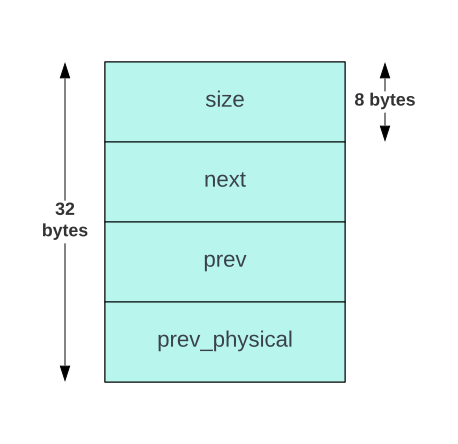
\includegraphics[width=\textwidth]{figures/blockheader_adap_general.png}
        \caption{Adapted general block header.}
        \label{fig:blockheader_adap_general}
    \end{subfigure}%
    \hfill
    \begin{subfigure}[b]{0.3\textwidth}
        \centering
        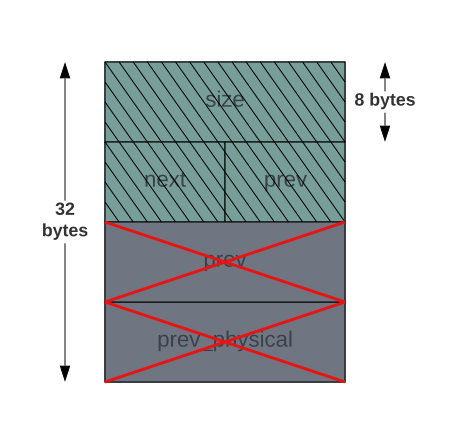
\includegraphics[width=\textwidth]{figures/blockheader_adap_optimized.png}
        \caption{Adapted optimized block header.}
        \label{fig:blockheader_adap_optimized}
    \end{subfigure}
    \caption{Overview of block header contents and adaptations. Dashed fields are only unused in the unused part of free blocks and crossed out fields are unused.}
    \label{fig:blockheader_adaptations}
\end{figure}

% TODO: Detta borde flyttas till discussion.
% A drawback of dividing the memory into only four second-levels per fist-level is that there is less chance that a block is closer to the size that we want to allocate. This could potentially lead to higher fragmentation, as there are fewer size classes of blocks available. However, this is generally not a problem...

%%% Local Variables:
%%% mode: latex
%%% TeX-master: "main"
%%% End:
